\documentclass{report}
\usepackage{graphicx}
\usepackage[round]{natbib}
%\usepackage[backend=biber]{biblatex}
%\addbibresource{bib.bib} % with extension
\usepackage{amsmath}

\begin{document}

\author{Hamid Shayestehmanesh}
\title{Exam Scheduler Application}
\maketitle
\tableofcontents
\newpage
\chapter{Introduction}
Examinations are essential because they compel students to learn. Without them, most students would not learn much. They would learn only subjects they are interested in and ignore the other topics, though they are significant in the modern age. 
\par
The way examinations are held critical. If they are taken too hard or too easy, the results cannot be trusted for judging and ranking students. Institutions should do their best to prepare a proper condition during exams for students to do their bests. However, they may have limitations in resources.
\chapter{Goal}
Our goal in this project is to design and implement an application for scheduling exams. Many institutions introduce some time slots during a few days or a week to place each exam in these time slots. For example,  they will take all the exams in one week, and exams must start at 8 A.M, 11 A.M or 2 in the afternoon. The apparent consideration for scheduling the exams are 1) All the students must be able to attend all of their exams 2) instructors also have to be available on their exams. Thus, an exam should not be held in its instructor's absence, nor two courses with the same instructor should be held at the same time. 


Possibly, a student may have two exams in one day or even in consecutive time slots, which feels unfair. This should be considered that universities have different limitation based on their policies. Our goal is to improve students' conditions while considering the policies of an institution. Our soft and hard constraints in this project will be explained entirely later.

\chapter{Overview}
In this chapter, we will review the input, the output, and the functionality of the application.

\section{Input}
Information given to the system contains all the possible time slots, courses' names, students, professors, and constraints. For the input format, please see the user manual.
% screen shot of different related parts
\section{Output}
The output is an exam's schedule on the predefined time slots, where it satisfies all the constraints given to the system. The system not only meets the hard constraints but also optimizes soft conditions. 
% screen shot of given times
\section{Functionality}
The most important functionalities are explained in the following.
\begin{itemize}
	\item[\textbf{Optimization}] {Our optimization engine is the primary significance of the application. Our engine schedule exams so that all the constraints are completely satisfied, and the soft constraints are minimized.
		\subsection{Constraints}
		\subsubsection{Hard Constrains}
			Hard Constraints must be met, and if they cannot be satisfied, then the problem has no answer.
			\begin{itemize}
				\item{No two courses of an instructor overlap.}
				\item{Students can attend all of their exams (No student has two exams at the same time).}
				\item{All exams will be held.}
				\item{No student has two exams back to back. For example, no one will have an exam on Sunday 8 A.M and Sunday 11 A.M however, one can have exams on 8 A.M and 2 P.M.}
				\item{No two major courses of current semester will be in same day, major courses are given to the system as input.}
			\end{itemize}
		\subsubsection{Soft Constrains}
						Soft constraints are constraints that we are trying to minimize. 
			\begin{itemize}
				\item{We minimize the number of instances that a student has two exams in one day. If a student has two exams in a day, it is counted as one conflict, but if a student has two exams in a day and two exams in another day, it's counted as two conflicts.}
				\item{We minimize the number of instances that a student has two exams in consecutive days.}
			\end{itemize}
			In this application, we consider the first soft constraint far more critical than the second one; therefore, we minimize the first one and then focus on the second one (This is not how the model is implemented, but it behaves like that).
		}
	\item[\textbf{Conflict Engine}] {There is a function which counts the three types of conflicts in a schedule. }
	\item[\textbf{Schedule Manually}] {Rather than scheduling automatically user can schedule the exams manually.}
\end{itemize}
\subsection{Database}
The database contains all the information we need. See the following diagram.


	\begin{figure}
		\center
			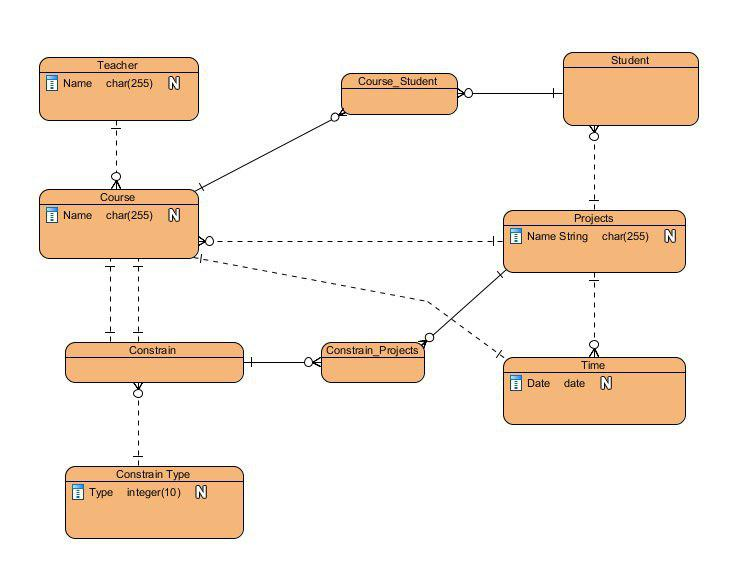
\includegraphics[width=4in]{db.jpg}
			\caption{Database ERD}
	\end{figure}

	

\chapter{Optimization Linear Model} 
In this chapter we take a look at the model designed to optimize our problem. $C, T$ are defined as the number of courses and the number of time slots.

\section{Tables}
This table can be constructed from the database.
\begin{itemize}
\item
{\textbf{Conf \big[ C \big]\big[ C \big]  \space =} \begin{tabular}{| c | c |} \hline
number of common students between class $i, j$ & if $i \neq j$ \\ \hline
0 & if $i = j$ \\ \hline
\end{tabular}}
\end{itemize}

\section{Variables}
Variables values' are assigned by the optimization solver.
\begin{itemize}
\item
{\textbf{SD \big[ C \big]\big[ C \big]  \space =}
\begin{tabular}{| c | c |} \hline
1 & course $i$ and $j$ being in same day for $i \neq j$ \\ \hline
0 & not being in same day \\ \hline
\end{tabular}}

\item{
\textbf{FS \big[ C \big]\big[ C \big]  \space =}
\begin{tabular}{| c | c |} \hline
1 & course $i$ and $j$ being in consecutive days for $i \neq j$ \\ \hline
0 & not being in consecutive day \\ \hline
\end{tabular}}

\item{
\textbf{CT \big[ C \big]\big[ T \big]  \space =}
\begin{tabular}{| c | c |} \hline
1 & if Course $c_i$ is decided to be in time $t_j$  \\ \hline
0 & if Course $c_i$ is decided not to be in time $t_j$ \\ \hline
\end{tabular}}


\end{itemize}

\section{Model}
\subsection{Objective}

\textbf{ \textit{Min:} } $\Sigma_{c_1}^{C} \Sigma_{c_2}^{C} SD[c_1][c_2] \times BIGM9 \times conf[c_1][c_2] + \Sigma_{c_1}^{C} \Sigma_{c_2}^{C} FD[c_1][c_2] \times BIGM6 \times conf[c_1][c_2]  $  \newline 

$BIGM9$ and $BIGM6$ are two big numbers which indicates the importance of each variable in our objective.
\subsection{Constraints and Explanations}
We add the following constraints to our linear model.
\begin{itemize}
\item{$\forall C$ \space $\Sigma_t^T CT_{ct} = 1$ \newline 
Exactly one time is assigned to each exam.}

\item{$\forall c_1 , c_2 , t $ \space if $c_1$, $c_2$ has conflicts $CT_{c_1 t} + CT_{c_2 t} \le 1$
	\newline 
	It assures that if two courses have any form of conflicts they will not be on same time. Conflict could, having common students, same instructor, or any other type of conflicts.
	 }

\item{$\forall c_1 , c_2 , t_1 , t_2$ \space if $c_1$, $c_2$ has conflicts and $t_1, t_2$ are consecutive times in a day, add the following constraints to the linear model.
	
	\begin{equation*}
		CT_{c_1 t_1} + CT_{c_2 t_2} \le 1
	\end{equation*}
	\begin{equation*}
		CT_{c_2 t_1} + CT_{c_1 t_2} \le 1 
	\end{equation*}
	Assures no student has consecutive exams.
	}

\item{$\forall c_1 , c_2 , t_1, t_2 $ \space if $c_1$, $c_2$ has students in common and $t_1 ,t_2 $ are in same day 
	\begin{equation*}
		CT_{c_1 t_1} + CT_{c_2 t_2} \le 1 + SD[c_1][c_2]		
	\end{equation*}
	\begin{equation*}
		CT_{c_1 t_2} + CT_{c_2 t_1} \le 1 + SD[c_1][c_2].
	\end{equation*} 
	This helps us count the number of students who have more than one exam in one day.
}


\item{$\forall c_1 ,  c_2 ,  t_1 , t_2$ \space if $c_1$, $c_2$ has conflicts and $t_1 , t_2$ are consecutive days 
	
	\begin{equation*}
		CT_{c_1 t_1} + CT_{c_2 t_2} \le 1 + FD[c_1][c_2]
	\end{equation*}
	\begin{equation*}
		CT_{c_2 t_1} + CT_{c_1 t_2} \le 1 + FD[c_1][c_2].
	\end{equation*}
	Finally, this helps us count the number of students who have exams in consecutive days. 	
  }

\end{itemize}
\section{Explanation}
FD and SD tables help us to calculate our objective cost.
\chapter{Manual}
Due to the fact that mother tongue of our costumer is Farsi, the user manual is written in a separate document in Farsi.

\end{document}